
\documentclass[usenames, dvipsnames, tikz]{standalone}

\usepackage{tikz}
\usetikzlibrary{calc}

\begin{document}
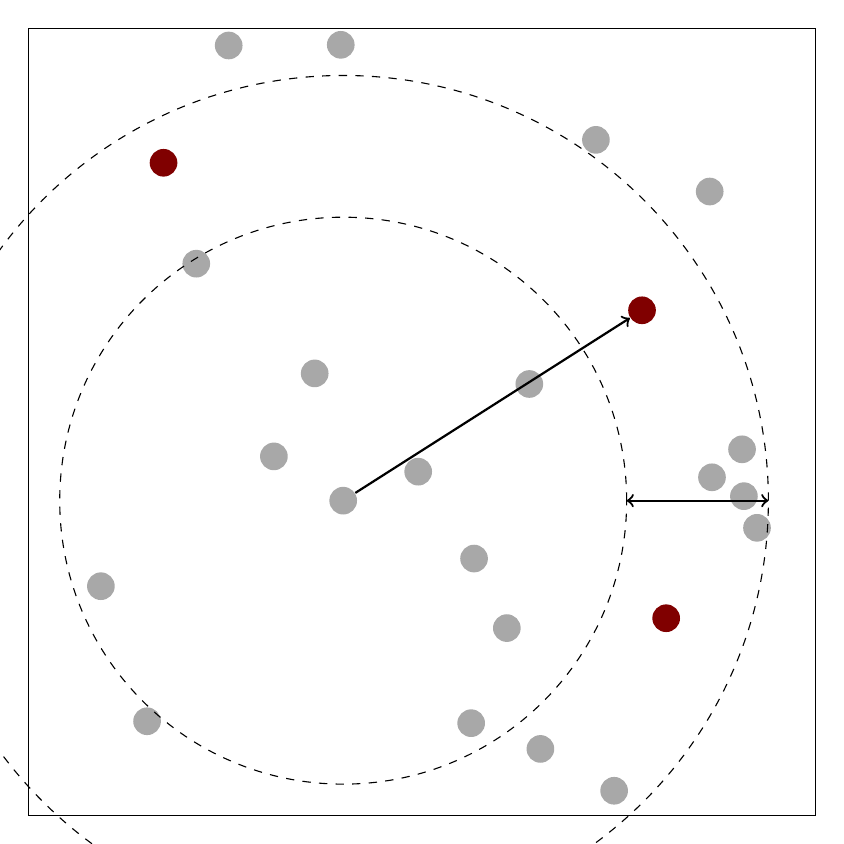
\begin{tikzpicture}[unconnected_neuron/.style={circle, inner sep=0,
    minimum size=10., fill=gray!68}, connected_neuron/.style={circle,
    inner sep=0, minimum size = 10., fill=Maroon}]

  %define neuron node style here!
  %define connected neuron node style here!

  \def \Edge {10.}
  \def \Distance {4.5}
  \def \Margin {0.9}


  \draw[use as bounding box] (0,0) rectangle (\Edge,\Edge);

  \node[unconnected_neuron]
  (Origin) at (4,4) {};

   \foreach \i in {1,2,...,20}{
    \pgfmathsetmacro{\X}{rnd*\Edge}
    \pgfmathsetmacro{\Y}{rnd*\Edge)}

    \node[unconnected_neuron] at
    (\X,\Y) {};
    }


  % \node[draw, circle, inner sep=0, minimum size=10, fill=gray!25]
  % (t_1) at (7,4) {};



  \node[connected_neuron] (Target) at
  ($(Origin) +(32.5:\Distance)$) {};

  \node[connected_neuron] (t1) at
  ($(Origin) +(118:\Distance+\Margin*0.4)$) {};

  \node[connected_neuron] (t2) at
  ($(Origin) +(340:\Distance-\Margin*0.15)$) {};

 

  \draw[dashed] (Origin) circle (\Distance+\Margin);
  \draw[dashed] (Origin) circle (\Distance-\Margin);

  \draw[thick, ->] (Origin) -- (Target);

  \draw[thick, <->] ($(Origin)+(\Distance-\Margin,0)$) --
  ($(Origin)+(\Distance+\Margin,0)$);

  %\draw[thick, dashed, ->] (Origin) -- ++(129:\Distance+\Margin*0.61);


  % \foreach \i in {1,2,...,10}{
  %   \pgfmathsetmacro{\ALPHA}{rnd*360.}
  %   \pgfmathsetmacro{\RADIUS}{rnd*(\Distance-\Margin)}

  %   \node[draw, circle, inner sep=0, minimum size=5., fill=gray!25] at
  %   ($(Origin) + (\ALPHA:\RADIUS)$) {};
  %   }

  % \foreach \i in {1,2,...,7}{
  %   %rnd from 0 to 1.
  %   \pgfmathsetmacro{\ALPHA}{rnd*360.}
  %   %rand from -1 to 1.
  %   \pgfmathsetmacro{\RADIUS}{rand*\Margin}

  %   \node[draw, circle, inner sep=0, minimum size=5., fill=red!25] at
  %   ($(Origin) + (\ALPHA:\Distance+\RADIUS)$) {};
  %   }

  % \foreach \i in {1,2,...,20}{
  %   \pgfmathsetmacro{\ALPHA}{rnd*360.}
  %   \pgfmathsetmacro{\RADIUS}{rnd*(3)}

  %   \node[draw, circle, inner sep=0, minimum size=5., fill=gray!25] at
  %   ($(Origin) + (\ALPHA:\Distance+\Margin+\RADIUS)$) {};
  %   }


\end{tikzpicture}
\end{document}
%%% Local Variables: 
%%% mode: latex
%%% TeX-master: t
%%% End: 
